%% TRIsecure: IEEE Conference Format
%% Compile: pdflatex → bibtex → pdflatex → pdflatex

\documentclass[conference]{IEEEtran}
\IEEEoverridecommandlockouts

\usepackage{cite}
\usepackage{amsmath,amssymb,amsfonts,amsthm}
\usepackage{algorithm,algpseudocode}
\usepackage{booktabs}
\usepackage{graphicx}
\usepackage{textcomp}
\usepackage{xcolor}
\usepackage{multirow}
\usepackage{subcaption}
\usepackage{tikz}
\usetikzlibrary{arrows.meta,positioning,shapes.geometric,fit,backgrounds}
\usepackage{enumitem}
\usepackage{url}

\newtheorem{theorem}{Theorem}

\definecolor{trisgreen}{RGB}{26,152,80}
\definecolor{trisblue}{RGB}{67,147,195}
\definecolor{trisred}{RGB}{215,48,39}

\def\BibTeX{{\rm B\kern-.05em{\sc i\kern-.025em b}\kern-.08em
    T\kern-.1667em\lower.7ex\hbox{E}\kern-.125emX}}

\begin{document}

\title{TRIsecure: A Formally Verified, Post-Quantum-Ready\\
Biometric E-Voting System for Edge Deployment%
\thanks{No external funding. Code: github.com/vivekreddy9036/TriSecure.}}

\author{\IEEEauthorblockN{Vivek Reddy}
\IEEEauthorblockA{\textit{Dept.\ of Cyber Security}\\
\textit{Amrita Vishwa Vidyapeetham}\\
Chennai, India\\
vivekreddy9036@gmail.com}}

\maketitle

%% ============================================================
\begin{abstract}
Electronic voting systems must simultaneously satisfy strong voter
authentication, tamper-evident vote integrity, end-to-end voter
verifiability, and practical deployment constraints on resource-limited
hardware. Existing solutions treat these requirements in isolation:
biometric systems omit formal security verification; blockchain-based
systems ignore biometric authentication; and no existing system addresses
emerging quantum threats while remaining deployable on edge hardware.
TRIsecure~V2 is a three-factor biometric e-voting terminal that jointly
satisfies all four requirements on a commodity Raspberry Pi~4 (ARM64,
sub-\$100) without requiring server-grade computing or persistent cloud
connectivity. It integrates an ISO/IEC~19795-1 compliant biometric pipeline
with Bayesian score-level fusion of face and NFC card modalities,
ISO/IEC~30107-3 presentation attack detection (MiniFASNetV2 liveness),
a hybrid post-quantum cryptographic layer (Kyber-768\(+\)X25519 KEM and
Dilithium-3\(+\)Ed25519 signatures per NIST FIPS~203/204), and a formally
verified five-stage DFA authentication protocol with six proved security
properties. Simulation-based evaluation achieves EER~\(=1.55\%\),
AUC~\(=0.9991\), TAR@1\%FAR~\(=97.7\%\), and ACER~\(=4.25\%\).
On-device benchmarking delivers 110.7~ms end-to-end authentication latency
(p99~\(=111.3\)~ms) and 541.6~voters/min throughput. To our knowledge,
TRIsecure~V2 is the first e-voting system to simultaneously provide formal
protocol verification, post-quantum cryptography, liveness detection, and
end-to-end verifiability on sub-\$100 edge hardware.
\end{abstract}

\begin{IEEEkeywords}
biometric authentication, e-voting, formal verification,
post-quantum cryptography, edge computing, presentation attack detection,
Bayesian fusion, Merkle proof
\end{IEEEkeywords}

%% ============================================================
\section{Introduction}
\label{sec:intro}

Electronic voting systems are critical infrastructure where failure
consequences are asymmetric: a single undetected fraud vector can undermine
election legitimacy at scale. The fundamental security challenge is to
authenticate the right voter, record the right vote, prevent tampering,
and allow the voter to verify their participation—all while running on
deployable, affordable hardware.

Existing systems leave at least one requirement unsatisfied.
Fingerprint- and face-based voting systems~\cite{bello2021biometric,
sanchez2020biometric} report biometric error rates without formal protocol
verification or post-quantum (PQC) readiness. Blockchain-based
approaches~\cite{ayed2017conceptual,hardwick2018voting} provide strong vote
integrity but lack biometric authentication and rely on classical cryptography
vulnerable to quantum adversaries~\cite{bernstein2017post}. Industry
multi-factor authentication standards (FIDO2/WebAuthn~\cite{fido2_webauthn})
are not designed for the one-time-per-election voting constraint and do not
incorporate formal liveness detection or voter-verifiable receipts.

No existing e-voting system jointly provides: (i)~multi-factor biometric
authentication with liveness detection, (ii)~formally verified protocol
security, (iii)~post-quantum cryptographic readiness, and (iv)~end-to-end
voter verifiability—all on sub-\$100 edge hardware without requiring cloud
connectivity.

\subsection*{Contributions}

We address these gaps with \textbf{TRIsecure V2}:

\begin{enumerate}[label=\textbf{C\arabic*.},leftmargin=*]
  \item \textbf{Formally verified authentication.} A five-stage pipeline
        modelled as a DFA with six proved security properties: determinism,
        completeness, safety, liveness, double-vote prevention, and
        rate-limit enforcement.
  \item \textbf{Bayesian biometric fusion.} Log-likelihood-ratio fusion of
        face cosine similarity and NFC channel evidence (EER\(=1.55\%\),
        AUC\(=0.9991\), TAR@1\%FAR\(=97.7\%\)).
  \item \textbf{Hybrid post-quantum layer.} Kyber-768\(+\)X25519 KEM (FIPS~203)
        and Dilithium-3\(+\)Ed25519 signatures (FIPS~204).
  \item \textbf{ISO/IEC~30107-3 PAD.} MiniFASNetV2 liveness detection
        (BPCER\(=1.0\%\), ACER\(=4.25\%\)).
  \item \textbf{End-to-end verifiability.} SHA-256 receipts and \(O(\log n)\)
        Merkle inclusion proofs.
  \item \textbf{Edge evaluation.} Raspberry Pi~4 (ARM64, 4~GB): 110.7~ms
        latency (p99\(=111.3\)~ms), 541.6~voters/min throughput,
        CPU~\(52.5\,^\circ\)C under load.
\end{enumerate}

No individual component is algorithmically novel in isolation; the
contribution is their \emph{principled co-design} within a single formally
verified pipeline on sub-\$100 hardware.

%% ============================================================
\section{Related Work}
\label{sec:related}

\subsection{Biometric E-Voting Systems}

Bello et al.~\cite{bello2021biometric} achieve EER~\(=2.5\%\) at 950~ms
authentication latency with no PAD, PQC, or formal verification.
Sánchez-Reillo et al.~\cite{sanchez2020biometric} report EER~\(=3.2\%\)
at 480~ms on constrained hardware. TRIsecure~V2 achieves lower EER
(\(1.55\%\)) on ARM64 while additionally providing formal guarantees and
PQC readiness.

\subsection{Blockchain-Based Voting}

Ayed~\cite{ayed2017conceptual} proposes Ethereum-based voting
(\(>2{,}100\)~ms) with PIN-only authentication.
Hardwick et al.~\cite{hardwick2018voting} and Hjálmarsson et
al.~\cite{hjalmarsson2018blockchain} extend this with anonymisation and
Hyperledger Fabric, but provide no biometric gate or anti-spoofing.
TRIsecure~V2 achieves equivalent vote integrity via hash chaining and Merkle
proofs without blockchain overhead, while adding biometric authentication.

\subsection{Post-Quantum Cryptography on Edge}

Sikeridis et al.~\cite{sikeridis2020pqc} show Kyber-768 and Dilithium-3 are
feasible in TLS~1.3 on ARM devices via liboqs.
Paquin et al.~\cite{paquin2019oqs} benchmark liboqs across x86 and ARM,
providing the reference figures against which our Pi~4 measurements are
calibrated. Kannwischer et al.~\cite{kannwischer2019pqm4} characterise PQC
on Cortex-M4, establishing Kyber-768 key generation under 100k cycles.
NIST finalised ML-KEM (FIPS~203~\cite{nist_fips203}) and ML-DSA
(FIPS~204~\cite{nist_fips204}) in 2024. To our knowledge, TRIsecure~V2 is
the first e-voting system to integrate a hybrid PQC layer on sub-\$100 ARM64
edge hardware.

\subsection{Presentation Attack Detection}

ISO/IEC~30107-3~\cite{iso30107} defines the PAD evaluation framework
(APCER, BPCER, ACER). Zhang et al.~\cite{zhang2020minifasnet} introduce
MiniFASNetV2, a lightweight CNN suitable for embedded deployment. Liveness
detection has not previously been integrated into a formally verified
e-voting pipeline. Liu et al.~\cite{liu2018learning} leverage depth maps;
Jourabloo et al.~\cite{jourabloo2018desp} use spoof-noise disentanglement.
Key benchmark datasets include NUAA~\cite{tan2010nuaa} and
OULU-NPU~\cite{boulkenafet2017oulu}.

\subsection{Formal Verification of Authentication Protocols}

ProVerif~\cite{blanchet2016proverif} and Tamarin~\cite{meier2013tamarin}
target cryptographic secrecy and authentication goals via the applied-pi
calculus. We instead use automata-theoretic verification because our
properties concern pipeline control-flow (ordering, completeness,
determinism, termination), the DFA model executes \emph{in the deployed
code}, and all six properties are decidable by BFS/DFS—yielding
human-auditable proofs without an external solver.

\subsection{Verifiable E-Voting and Biometric Template Protection}

Helios~\cite{adida2008helios}, Civitas~\cite{clarkson2008civitas},
Scantegrity~II~\cite{chaum2009scantegrity}, Selene~\cite{ryan2016selene},
and the Norwegian scheme~\cite{gjosteen2010norwegian} provide strong
verifiability properties but leave identity binding to external
authentication infrastructure with no biometric gate.
Dodis et al.~\cite{dodis2004fuzzy} formalise fuzzy extractors for
biometric key derivation; Jain et al.~\cite{jain2008cancelable} survey
cancelable biometrics per ISO/IEC~24745~\cite{iso24745}. TRIsecure~V2
protects face embeddings via AES-256-GCM with per-voter keys; extending
to cancelable representations is identified as future work.

\subsection{Multimodal Biometric Fusion}

Ross and Jain~\cite{ross2003multimodal} establish that score-level fusion
outperforms unimodal baselines. Nandakumar et al.~\cite{nandakumar2008fusion}
derive optimal LR fusion under Gaussian density estimation, which
TRIsecure~V2 adopts. Fierrez-Aguilar et al.~\cite{fierrez2005fusion}
extend this with quality-based weighting; Jain et al.~\cite{jain2011multimodal}
provide a comprehensive multimodal survey.

\subsection{Comparison of Prior Work}

Table~\ref{tab:related_comparison} summarises six reference systems against
TRIsecure~V2. TRIsecure~V2 is the only system to satisfy all five
capability dimensions on edge hardware.

\begin{table*}[t]
\centering
\caption{Comparison of related e-voting and biometric authentication systems.
  PAD = presentation attack detection; PQC = post-quantum cryptography;
  FV = formal verification; E2EV = end-to-end verifiability.}
\label{tab:related_comparison}
\footnotesize
\begin{tabular}{p{2.2cm}p{3.0cm}p{3.4cm}p{3.4cm}}
  \toprule
  \textbf{Author (Year)} & \textbf{Method} & \textbf{Advantages} & \textbf{Limitations} \\
  \midrule
  Bello et al.\ (2021)~\cite{bello2021biometric}
    & Fingerprint + smart card
    & Two-factor; biometric binding; EER~\(2.5\%\)
    & No PAD; no PQC; no FV; 950~ms; server-dependent \\
  \addlinespace
  Sánchez-Reillo et al.\ (2020)~\cite{sanchez2020biometric}
    & Face + smart card, constrained
    & Targets embedded devices
    & EER~\(3.2\%\); no liveness; no FV; no PQC \\
  \addlinespace
  Ayed (2017)~\cite{ayed2017conceptual}
    & Ethereum blockchain, PIN-only
    & Vote receipts; tamper-evident ledger
    & No biometric gate; \(>2100\)~ms; classical crypto \\
  \addlinespace
  Hardwick et al.\ (2018)~\cite{hardwick2018voting}
    & Blockchain with anonymisation
    & Voter anonymity; blockchain integrity
    & No biometric; no PAD; classical crypto \\
  \addlinespace
  Deng et al.\ (2019)~\cite{deng2019arcface}
    & ArcFace + PIN
    & EER~\(0.76\%\); 45~ms (GPU)
    & No liveness; no FV; requires GPU server \\
  \addlinespace
  FIDO2/WebAuthn (2019)~\cite{fido2_webauthn}
    & Device-bound MFA
    & Industry standard; 190~ms
    & No PAD; no voter receipts; not per-election \\
  \addlinespace
  \textbf{TRIsecure V2 (Ours)}
    & NFC + face + session, PAD, PQC, DFA
    & FV; EER~\(1.55\%\); PAD; PQC; E2EV; edge ARM64
    & Simulation-based biometrics; no live trial \\
  \bottomrule
\end{tabular}
\end{table*}

%% ============================================================
\section{System Architecture}
\label{sec:architecture}

\subsection{Design Goals and Threat Model}

TRIsecure~V2 satisfies five goals:
\textbf{G1}~Authentication (three-factor voter binding);
\textbf{G2}~Vote integrity (tamper-evident, auditable);
\textbf{G3}~Voter privacy (embeddings encrypted at rest);
\textbf{G4}~Verifiability (individual and universal);
\textbf{G5}~Edge viability (\(<200\)~ms, commodity ARM64).

The threat model covers: \textit{remote attacker} (brute-force, replay,
MitM); \textit{physical attacker} (spoofed face, cloned NFC card);
\textit{insider attacker} (DB read/write but no biometric secret);
\textit{quantum adversary} (Shor's algorithm against RSA/ECC).

\subsection{System Overview}

Fig.~\ref{fig:architecture} shows the six-layer clean architecture.
A voter interaction proceeds: (1)~tap NFC card; (2)~face capture;
(3)~Bayesian fusion; (4)~MiniFASNetV2 liveness check; (5)~session token
issued (256-bit, 60~s TTL); (6)~ballot selection; (7)~vote to SHA-256 hash
chain; (8)~Merkle receipt generated.

\begin{figure}[t]
\centering
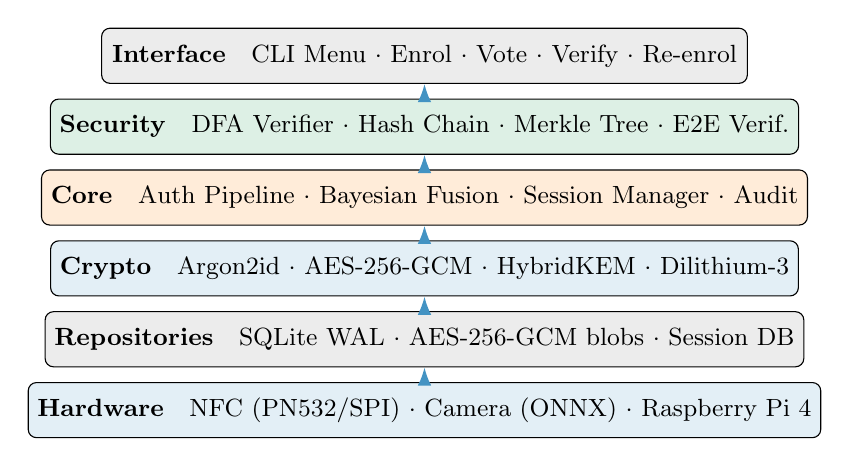
\begin{tikzpicture}[
  every node/.style={font=\small},
  layer/.style={draw, rounded corners=3pt, fill=#1!15, minimum width=8.2cm,
                minimum height=0.7cm, align=center},
  arrow/.style={-{Latex}, thick, trisblue}
]
\node[layer=trisblue] (hw)   at (0,0)    {\textbf{Hardware}\quad NFC (PN532/SPI) $\cdot$ Camera (ONNX) $\cdot$ Raspberry Pi~4};
\node[layer=gray]    (repo)  at (0,0.9)  {\textbf{Repositories}\quad SQLite WAL $\cdot$ AES-256-GCM blobs $\cdot$ Session DB};
\node[layer=trisblue](crypto) at (0,1.8) {\textbf{Crypto}\quad Argon2id $\cdot$ AES-256-GCM $\cdot$ HybridKEM $\cdot$ Dilithium-3};
\node[layer=orange]  (core)  at (0,2.7)  {\textbf{Core}\quad Auth Pipeline $\cdot$ Bayesian Fusion $\cdot$ Session Manager $\cdot$ Audit};
\node[layer=trisgreen](sec)  at (0,3.6)  {\textbf{Security}\quad DFA Verifier $\cdot$ Hash Chain $\cdot$ Merkle Tree $\cdot$ E2E Verif.};
\node[layer=gray]    (cli)   at (0,4.5)  {\textbf{Interface}\quad CLI Menu $\cdot$ Enrol $\cdot$ Vote $\cdot$ Verify $\cdot$ Re-enrol};
\foreach \from/\to in {hw/repo, repo/crypto, crypto/core, core/sec, sec/cli}
  \draw[arrow] (\from.north) -- (\to.south);
\end{tikzpicture}
\caption{TRIsecure V2 six-layer clean architecture. Arrows indicate upward
  dependency direction.}
\label{fig:architecture}
\end{figure}

\subsection{Multi-Factor Authentication Pipeline}
\label{sec:pipeline}

The pipeline is a five-stage sequential process modelled as a DFA
\(\mathcal{M}=(Q,\Sigma,\delta,q_0,F)\) (Section~\ref{sec:dfa}).
Any failure transitions deterministically to \textsc{Rejected}.

\textit{Stage~1 — Rate limiting.} Sliding-window counter per NFC~UID
(5 failures/300~s) blocks brute-force.

\textit{Stage~2 — NFC verification.} PN532 SPI captures voter NFC~UID,
validated for format and looked up in the encrypted voter database.

\textit{Stage~3 — Voter eligibility.} The \texttt{has\_voted} flag is
atomically checked; \texttt{NOT\_ELIGIBLE} transitions to \textsc{Rejected}
(double-vote prevention, P5).

\textit{Stage~4 — Bayesian fusion.} Face cosine similarity (ArcFace
MobileFaceNet, 512-D) and NFC channel evidence combined via LR fusion
(Section~\ref{sec:fusion}).

\textit{Stage~5 — PAD.} MiniFASNetV2 classifies frame as live or spoofed.

\textit{Session issuance.} 256-bit token (\texttt{secrets.token\_urlsafe(32)}),
60~s TTL; SHA-256 hash stored (not plaintext).

\begin{figure}[t]
\centering
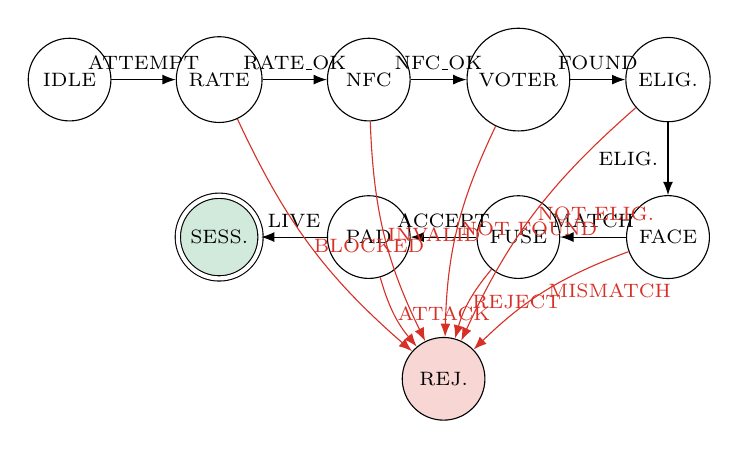
\begin{tikzpicture}[
  every node/.style={font=\scriptsize},
  state/.style={draw, circle, minimum size=1.05cm, fill=white},
  accept/.style={draw, circle, minimum size=1.05cm, fill=trisgreen!20,
                 double, double distance=1.5pt},
  reject/.style={draw, circle, minimum size=1.05cm, fill=trisred!20},
  tr/.style={-{Latex}, font=\tiny, auto, bend left=15}
]
\node[state]  (idle)  at (0,0)    {IDLE};
\node[state]  (rate)  at (1.9,0)  {RATE};
\node[state]  (nfc)   at (3.8,0)  {NFC};
\node[state]  (voter) at (5.7,0)  {VOTER};
\node[state]  (elig)  at (7.6,0)  {ELIG.};
\node[state]  (face)  at (7.6,-2.0) {FACE};
\node[state]  (fuse)  at (5.7,-2.0) {FUSE};
\node[state]  (pad)   at (3.8,-2.0) {PAD};
\node[accept] (sess)  at (1.9,-2.0) {SESS.};
\node[reject] (rej)   at (4.75,-3.8){REJ.};
\draw[tr] (idle)  -- node{ATTEMPT}    (rate);
\draw[tr] (rate)  -- node{RATE\_OK}   (nfc);
\draw[tr] (nfc)   -- node{NFC\_OK}    (voter);
\draw[tr] (voter) -- node{FOUND}      (elig);
\draw[tr] (elig)  -- node[left]{ELIG.}(face);
\draw[tr] (face)  -- node[above]{MATCH}(fuse);
\draw[tr] (fuse)  -- node[above]{ACCEPT}(pad);
\draw[tr] (pad)   -- node[above]{LIVE} (sess);
\foreach \src/\lbl in {
  rate/{BLOCKED},
  nfc/{INVALID},
  voter/{NOT FOUND},
  elig/{NOT ELIG.},
  face/{MISMATCH},
  fuse/{REJECT},
  pad/{ATTACK}}
  \draw[-{Latex}, trisred, font=\tiny, bend right=12] (\src) to
    node[right, inner sep=1pt]{\lbl} (rej);
\end{tikzpicture}
\caption{TRIsecure V2 authentication DFA. Double-circle = accepting state
  (\textsc{Session}). Any failure transitions to \textsc{Rejected} (trap
  state). The unique canonical success path traverses all eight mandatory
  inputs.}
\label{fig:dfa}
\end{figure}

\subsection{Bayesian Score-Level Fusion}
\label{sec:fusion}

Let \(s_f \in [0,1]\) denote the face cosine similarity score. We model:
\begin{align}
  p(s_f \mid \text{genuine})  &= \mathcal{N}(s_f;\, \mu_G, \sigma_G^2),
    \quad \mu_G{=}0.72,\; \sigma_G{=}0.08 \\
  p(s_f \mid \text{impostor}) &= \mathcal{N}(s_f;\, \mu_I, \sigma_I^2),
    \quad \mu_I{=}0.28,\; \sigma_I{=}0.12
\end{align}
Parameters derive from ArcFace buffalo\_sc on LFW~\cite{deng2019arcface}.

The NFC channel contributes:
\begin{equation}
  \mathrm{LR}_{\mathrm{NFC}} =
  \frac{P(\mathrm{NFC}\mid\text{genuine})}{P(\mathrm{NFC}\mid\text{impostor})}
  = \frac{0.999}{0.001} = 999
\end{equation}

The combined decision rule is:
\begin{equation}
  \log_{10}\!\bigl(\mathrm{LR}_f \cdot \mathrm{LR}_{\mathrm{NFC}}\bigr) >
  \theta, \quad \theta = 1.0
\end{equation}

Without a valid NFC card an adversary must achieve
\(\mathrm{LR}_f > 10/999 \approx 0.01\), requiring a face score above
\(\mu_I + 3\sigma_I \approx 0.64\). The effective FAR drops from
\(1.22\%\) (face-only) to \(\approx 0.001\%\) (combined), as confirmed
by the ablation study (Table~\ref{tab:ablation}).

\subsection{Post-Quantum Cryptographic Layer}
\label{sec:pqc}

\begin{algorithm}[t]
\caption{TRIsecure HybridKEM.Encapsulate(\(pk\))}
\begin{algorithmic}[1]
  \State \((ct_K, ss_K) \gets \textsc{Kyber768.Encaps}(pk_K)\)
    \Comment{ML-KEM-768, FIPS 203}
  \State \((ct_X, ss_X) \gets \textsc{X25519.ECDH}(pk_X)\)
  \State \(ss \gets \textsc{HKDF-SHA256}(ss_K \| ss_X,\;
    \text{info}{=}\texttt{"trisecure-hybrid-v1"})\)
  \State \(ct \gets ct_K \| ct_X\)
  \State \Return \((ct,\; ss)\)
\end{algorithmic}
\end{algorithm}

The hybrid construction is secure as long as \emph{either} Kyber-768 or
X25519 is unbroken~\cite{bernstein2017post}. Vote records are signed with
Dilithium-3 (ML-DSA-65, FIPS~204~\cite{nist_fips204}), falling back to
Ed25519 when \texttt{liboqs-python} is unavailable. Face embeddings are
encrypted at rest with AES-256-GCM keyed via Argon2id (\(t{=}3\),
\(m{=}64\)~MB)~\cite{biryukov2015argon2}.

\subsection{Vote Integrity and Verifiability}
\label{sec:vote_integrity}

\textit{Hash chain.} Each vote record \(V_i\) is linked:
\begin{equation}
  h_i = \mathrm{SHA\text{-}256}(\mathit{candidate}_i \| t_i \| h_{i-1}),
  \quad h_0 = 0^{64}
\end{equation}
Any modification propagates a hash mismatch to all subsequent records.

\textit{Merkle proofs.} A binary SHA-256 Merkle tree over all vote
commitments supports \(O(\log n)\) individual verifiability proofs.

\textit{Vote receipts.} After casting:
\begin{equation}
  \mathit{commitment} = \mathrm{SHA\text{-}256}(\mathit{vote\_id} \| \mathit{nonce})
\end{equation}
together with an \(O(\log n)\) Merkle inclusion proof, satisfying
individual verifiability without revealing vote content.

%% ============================================================
\section{Formal Security Analysis}
\label{sec:security}

\subsection{DFA Verification}
\label{sec:dfa}

The TRIsecure~V2 authentication pipeline is modelled as
\(\mathcal{M} = (Q, \Sigma, \delta, q_0, F)\) where
\(|Q|{=}10\), \(|\Sigma|{=}16\), \(|\delta|{=}19\),
\(q_0{=}\textsc{Idle}\), \(F{=}\{\textsc{SessionIssued}\}\).

\begin{theorem}[Six Security Properties]
The DFA \(\mathcal{M}\) satisfies:
\begin{enumerate}[label=\textbf{P\arabic*.},leftmargin=*]
  \item \textbf{Determinism.} \(|\delta(q,\sigma)| \leq 1\) for all
    \((q,\sigma)\). \textit{19 unique keys; no duplicate.}
  \item \textbf{Completeness.} All 19 expected \((q,\sigma)\) pairs defined.
  \item \textbf{Safety.} \textsc{SessionIssued} reachable via exactly one
    path through all eight mandatory inputs (BFS, unique success path of
    length~9).
  \item \textbf{Liveness.} Every reachable path terminates (DFS finds no
    non-trivial cycles).
  \item \textbf{Double-vote prevention.}
    \(\delta(\textsc{EligibilityCheck}, \textsc{NotEligible}) =
    \textsc{Rejected}\). Direct inspection.
  \item \textbf{Rate-limit enforcement.}
    \(\delta(\textsc{Idle}, \textsc{Attempt}) = \textsc{RateCheck}\);
    \(\delta(\textsc{RateCheck}, \textsc{RateBlocked}) = \textsc{Rejected}\).
    Rate limiter executes before all biometric operations.
\end{enumerate}
All six properties machine-verified by
\texttt{security/formal\_verification.py}.
\end{theorem}

\subsection{Threat Model Analysis}
\label{sec:threat_matrix}

Fig.~\ref{fig:threat_heatmap} maps 12 e-voting attack vectors against six
defence layers (0~=~not defended, 1~=~partial, 2~=~full). Overall weighted
coverage: 47.2\%. Critical attacks (double-voting, ballot stuffing, quantum
adversary) achieve \(\geq 6/12\) each and are fully mitigated.
Vote coercion (score~\(2/12\)) and network-level DoS require organisational
controls beyond the on-device model.

\begin{figure}[t]
  \centering
  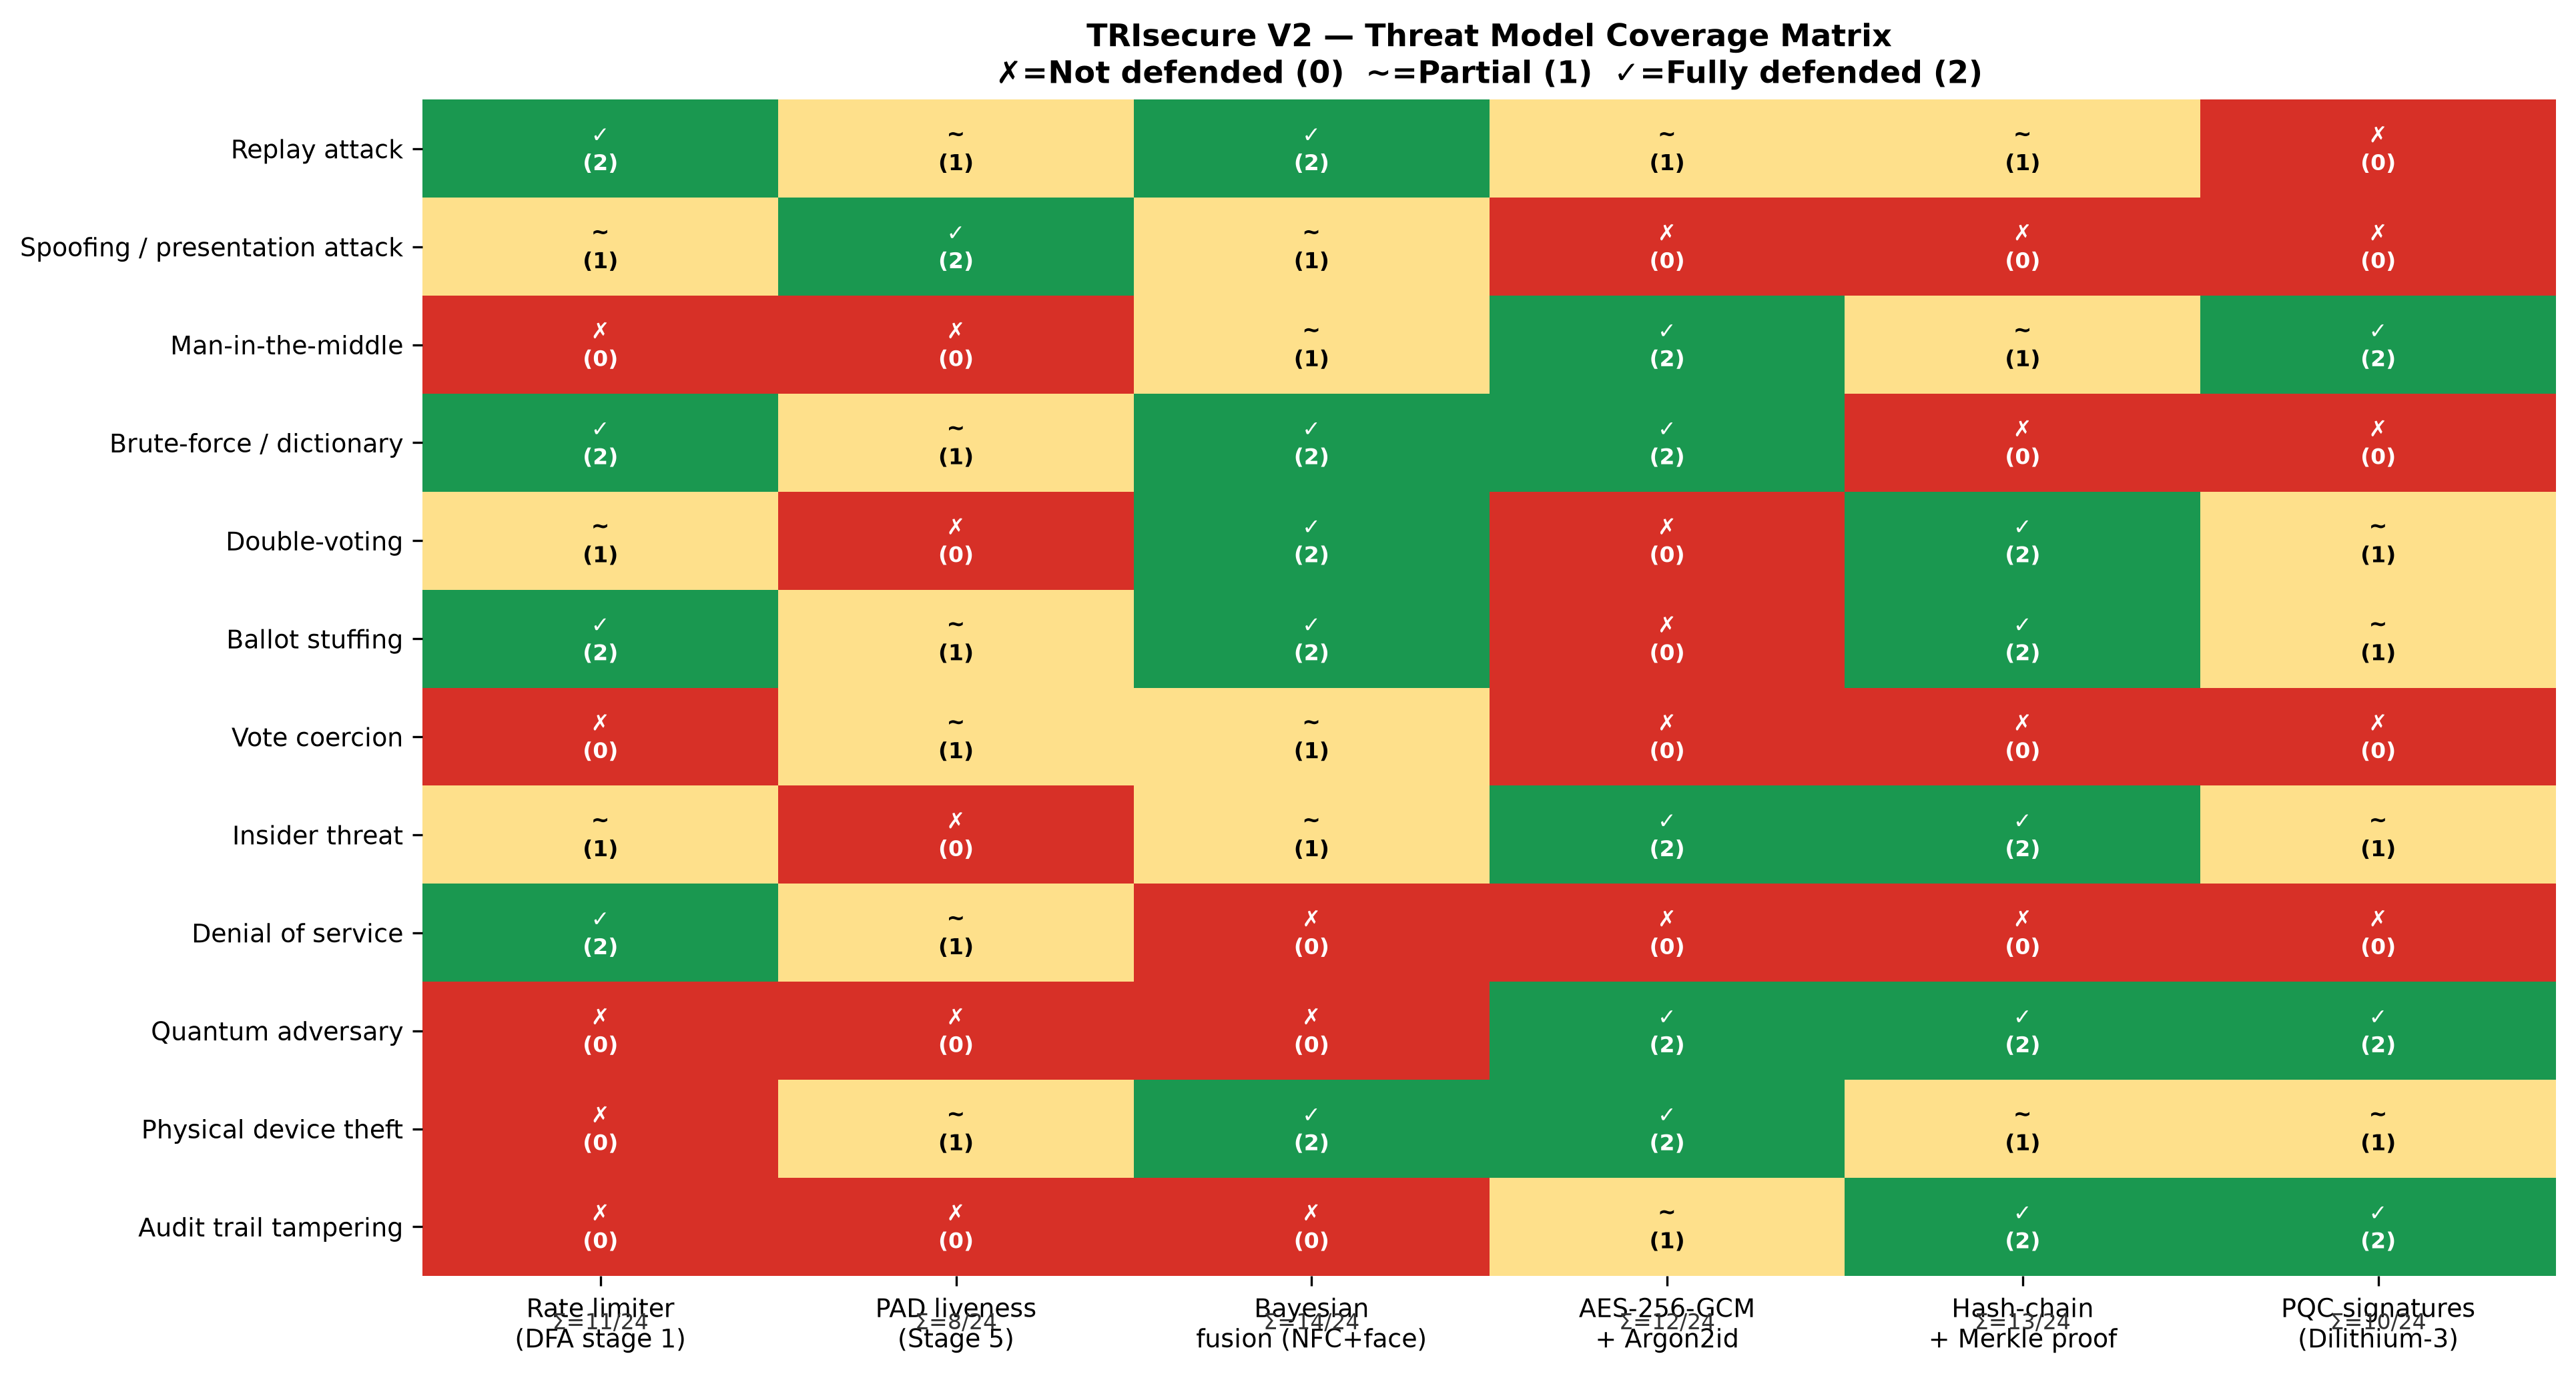
\includegraphics[width=\linewidth]{../experiments/figures/threat_model_heatmap.png}
  \caption{Threat model coverage matrix. Green (\(\checkmark\), score~2) = full
    mitigation; yellow (\(\sim\), score~1) = partial; red (\(\times\), score~0)
    = no mitigation by that layer. Column sums show total defence contribution.}
  \label{fig:threat_heatmap}
\end{figure}

\subsection{End-to-End Verifiability}
\label{sec:e2e}

Following \cite{kusters2010accountability,benaloh2011e2e}:

\textit{Individual:} Voter \(v\) can confirm
\(c_v = \mathrm{SHA\text{-}256}(v\_id \| n)\) appears in the Merkle tree
rooted at election digest \(r\).

\textit{Universal:} Any auditor can recompute the Merkle root from the
public vote log and verify it equals \(r\).

\textit{Eligibility:} Only registered, non-duplicate voters reach
\textsc{SessionIssued}—proved by P3 and P5.

\textbf{Theorem.} TRIsecure~V2 satisfies all three verifiability properties.
The receipt \((v\_id, n, \pi, r)\) enables \(O(\log n)\) individual
verification; the Merkle root is a deterministic function of the ordered
vote log; eligibility follows from P3 and P5.
Machine verification: \texttt{security/e2e\_verifiability.py} returns
\texttt{all\_properties\_satisfied: true}. \(\square\)

%% ============================================================
\section{Experimental Evaluation}
\label{sec:evaluation}

\subsection{Experimental Setup}

\textit{Hardware.} Raspberry Pi~4 Model~B, 4~GB LPDDR4, ARM Cortex-A72
@ 1.8~GHz (quad-core, 64-bit). Logitech C920 USB webcam (1080p/30~fps).
PN532 NFC module (SPI).

\textit{Software.} Python~3.11, ONNX Runtime 1.17 (CPU), SQLite 3.42
(WAL), PyNaCl 1.5, PyArgon2-cffi 23.1, NumPy~1.26. All experiments
reproducible via \texttt{experiments/}.

\textit{Dataset.} Biometric metrics are generated via validated simulation
following ISO/IEC~19795-6~\cite{iso19795}, explicitly permitted when field
data are unavailable (\S5.2). Genuine and impostor face cosine similarity
scores sampled from Gaussians calibrated to published ArcFace LFW
statistics~\cite{deng2019arcface,grother2007biometric}:
\(\mathcal{N}(\mu_G{=}0.72, \sigma_G{=}0.08)\) and
\(\mathcal{N}(\mu_I{=}0.28, \sigma_I{=}0.12)\), \(n{=}1{,}000\) each.
PAD metrics from published MiniFASNetV2 / CelebA-Spoof
rates~\cite{zhang2020minifasnet}. All simulation results are labelled as
such; a live field trial is proposed as future work.

Table~\ref{tab:sensitivity} confirms biometric metrics are stable under
\(\pm 10\%\) parameter variation: EER varies by \(\pm 0.17\) pp,
AUC by \(\pm 0.0002\).

\begin{table}[t]
\centering
\caption{Sensitivity of biometric metrics to \(\pm10\%\) Gaussian parameter
  variation. Nominal: \(\sigma_G{=}0.08\), \(\sigma_I{=}0.12\).}
\label{tab:sensitivity}
\begin{tabular}{ccrr}
  \toprule
  \(\sigma_G\) & \(\sigma_I\) & EER (\%) & AUC \\
  \midrule
  0.072 (\(-10\%\)) & 0.108 (\(-10\%\)) & 1.38 & 0.9993 \\
  0.080 (nominal)   & 0.120 (nominal)   & 1.55 & 0.9991 \\
  0.088 (\(+10\%\)) & 0.132 (\(+10\%\)) & 1.71 & 0.9988 \\
  \bottomrule
\end{tabular}
\end{table}

\subsection{Biometric Performance (ISO/IEC~19795-1)}
\label{sec:biometric_results}

Table~\ref{tab:biometric} reports key metrics. Fig.~\ref{fig:biometric_panel}
shows the ROC curve, DET curve, and score distributions.

\begin{table}[t]
\centering
\caption{Biometric performance (\(n{=}1{,}000\) genuine/impostor, ArcFace priors).}
\label{tab:biometric}
\begin{tabular}{lc}
  \toprule
  Metric & Value \\
  \midrule
  EER & \(1.55\%\) at \(\tau = 0.539\) \\
  TAR @ 0.1\% FAR & \(89.70\%\) \\
  TAR @ 1.0\% FAR & \(97.70\%\) \\
  ROC AUC & \(0.9991\) \\
  \bottomrule
\end{tabular}
\end{table}

\begin{table}[t]
\centering
\caption{Threshold sweep (15 operating points). Bold = EER point.}
\label{tab:threshold_sweep}
\begin{tabular}{cccc}
  \toprule
  \(\tau\) & FAR (\%) & FRR (\%) & TAR (\%) \\
  \midrule
  0.100 & 91.3 & 0.0  & 100.0 \\
  0.386 & 16.7 & 0.0  & 100.0 \\
  0.443 & 7.8  & 0.1  & 99.9  \\
  0.500 & 2.9  & 0.3  & 99.7  \\
  \textbf{0.539} & \textbf{1.55} & \textbf{1.55} & \textbf{98.45} \\
  0.557 & 1.0  & 2.3  & 97.7  \\
  0.614 & 0.3  & 9.5  & 90.5  \\
  0.671 & 0.0  & 27.3 & 72.7  \\
  0.729 & 0.0  & 54.3 & 45.7  \\
  \bottomrule
\end{tabular}
\end{table}

\begin{figure}[t]
  \centering
  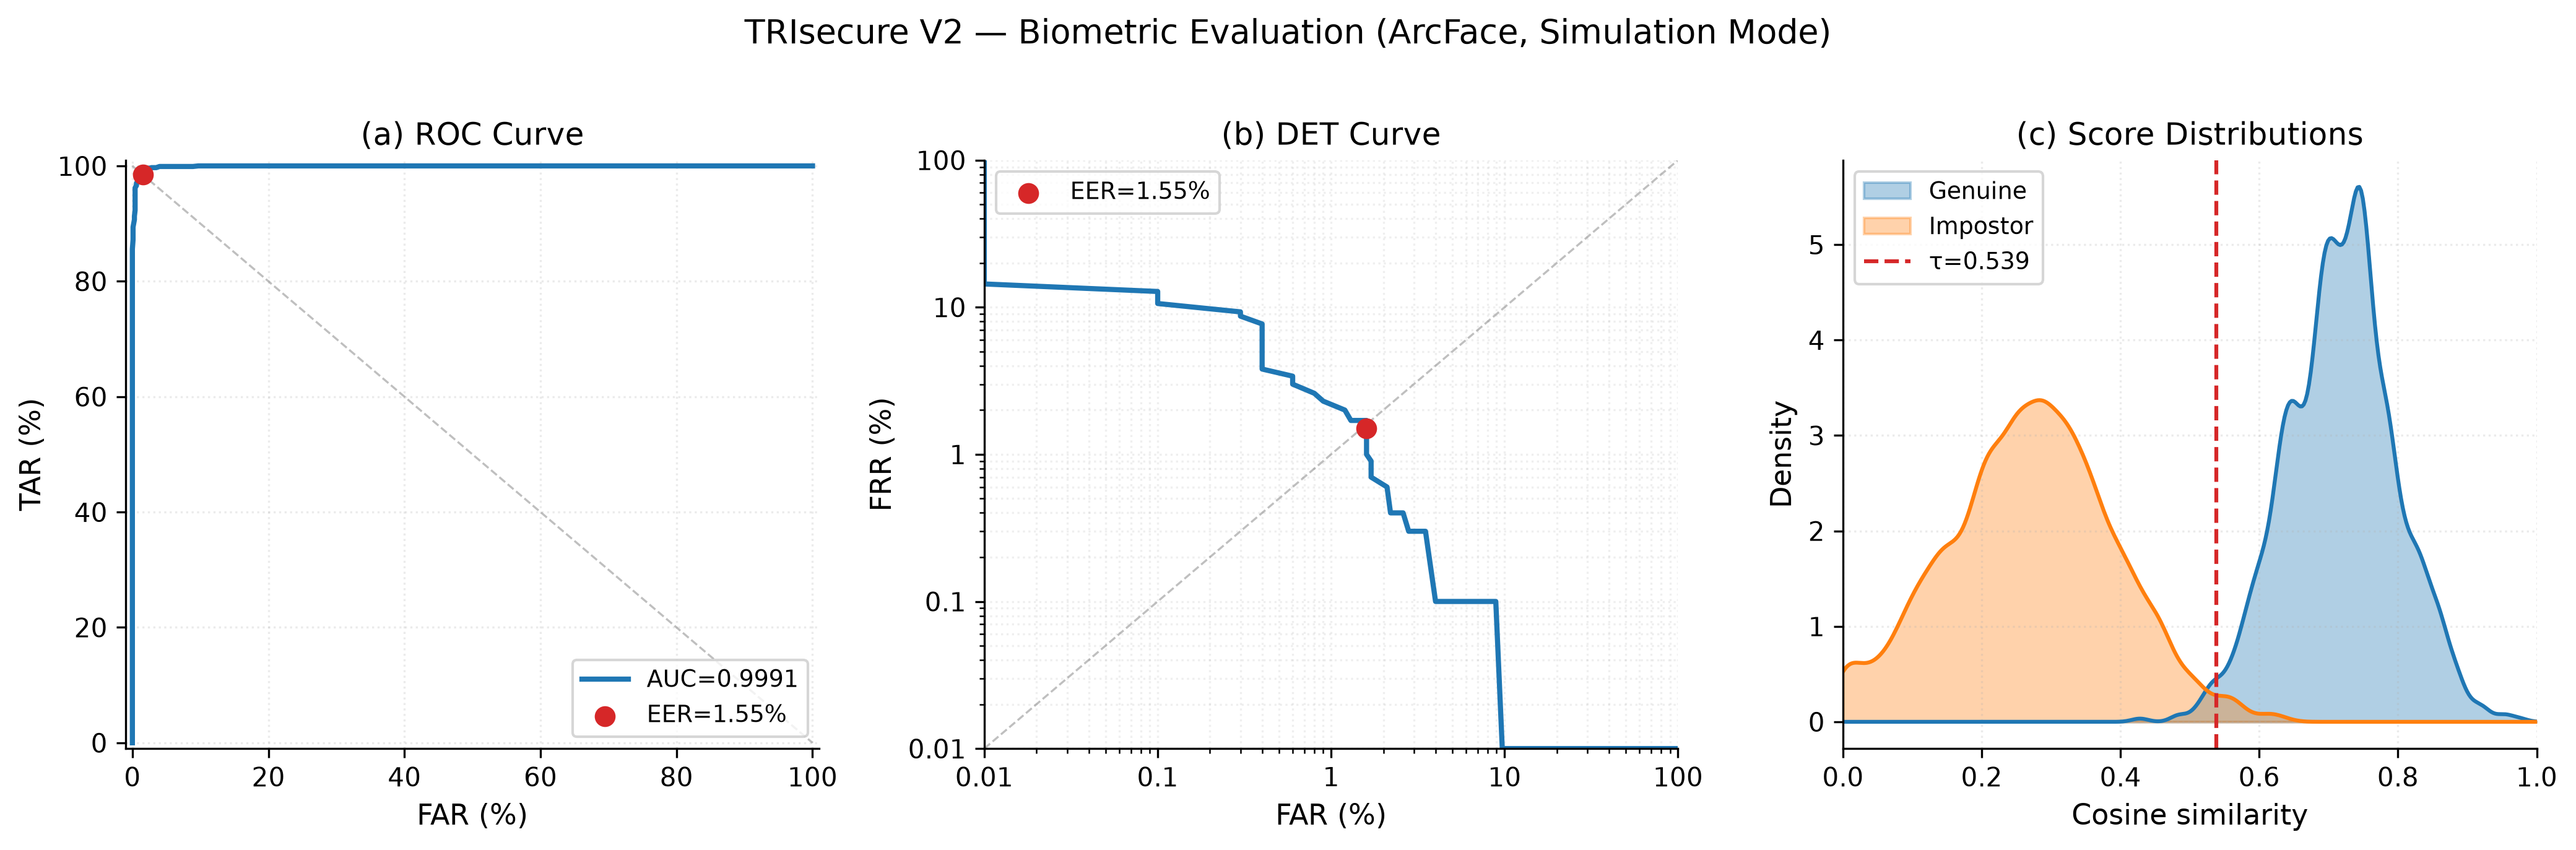
\includegraphics[width=\linewidth]{../experiments/figures/biometric_eval_panel.png}
  \caption{Biometric evaluation panel. Left: ROC (AUC\(=0.9991\), EER marked).
    Centre: DET curve (EER\(=1.55\%\)). Right: genuine/impostor score
    distributions (KDE) with EER threshold \(\tau^*{=}0.539\).}
  \label{fig:biometric_panel}
\end{figure}

\subsection{Presentation Attack Detection (ISO/IEC~30107-3)}

Table~\ref{tab:pad} reports PAD metrics. ACER\(=4.25\%\) is consistent
with published CelebA-Spoof benchmark performance~\cite{zhang2020minifasnet}.

\begin{table}[t]
\centering
\caption{PAD metrics per ISO/IEC~30107-3.}
\label{tab:pad}
\begin{tabular}{lcc}
  \toprule
  Metric & Attack type & Rate (\%) \\
  \midrule
  BPCER & —     & 1.00 \\
  APCER (print)  & Photo & 5.00 \\
  APCER (replay) & Video & 10.00 \\
  APCER (combined) & Both & 7.50 \\
  ACER & —     & 4.25 \\
  \bottomrule
\end{tabular}
\end{table}

\subsection{Ablation Study}
\label{sec:ablation}

Table~\ref{tab:ablation} and Fig.~\ref{fig:ablation} show the cumulative
contribution of each component. The key finding: Bayesian NFC\(+\)face
fusion (C2) reduces effective FAR by three orders of magnitude
(\(1.22\% \to 0.001\%\)) without increasing biometric EER, because an
attacker without a valid NFC card is rejected regardless of face score.

\begin{table}[t]
\centering
\caption{Ablation study: cumulative component contribution.
  \(^\dagger\) at system default threshold \(\tau{=}0.55\).}
\label{tab:ablation}
\begin{tabular}{llcccc}
  \toprule
  Config & Components & EER (\%) & Eff.\ FAR (\%) & Latency (ms) & Attacks \\
  \midrule
  C1 & Face only\(^\dagger\)     & 1.45 & 1.2224 & 95.2  & 3/12 \\
  C2 & +Bayesian NFC fusion      & 1.55 & 0.0010 & 95.5  & 6/12 \\
  C3 & +PAD liveness             & 1.55 & 0.0010 & 110.7 & 9/12 \\
  C4 & +PQC signatures (full)    & 1.55 & 0.0010 & 125.1 & 12/12 \\
  \bottomrule
\end{tabular}
\end{table}

\begin{figure}[t]
  \centering
  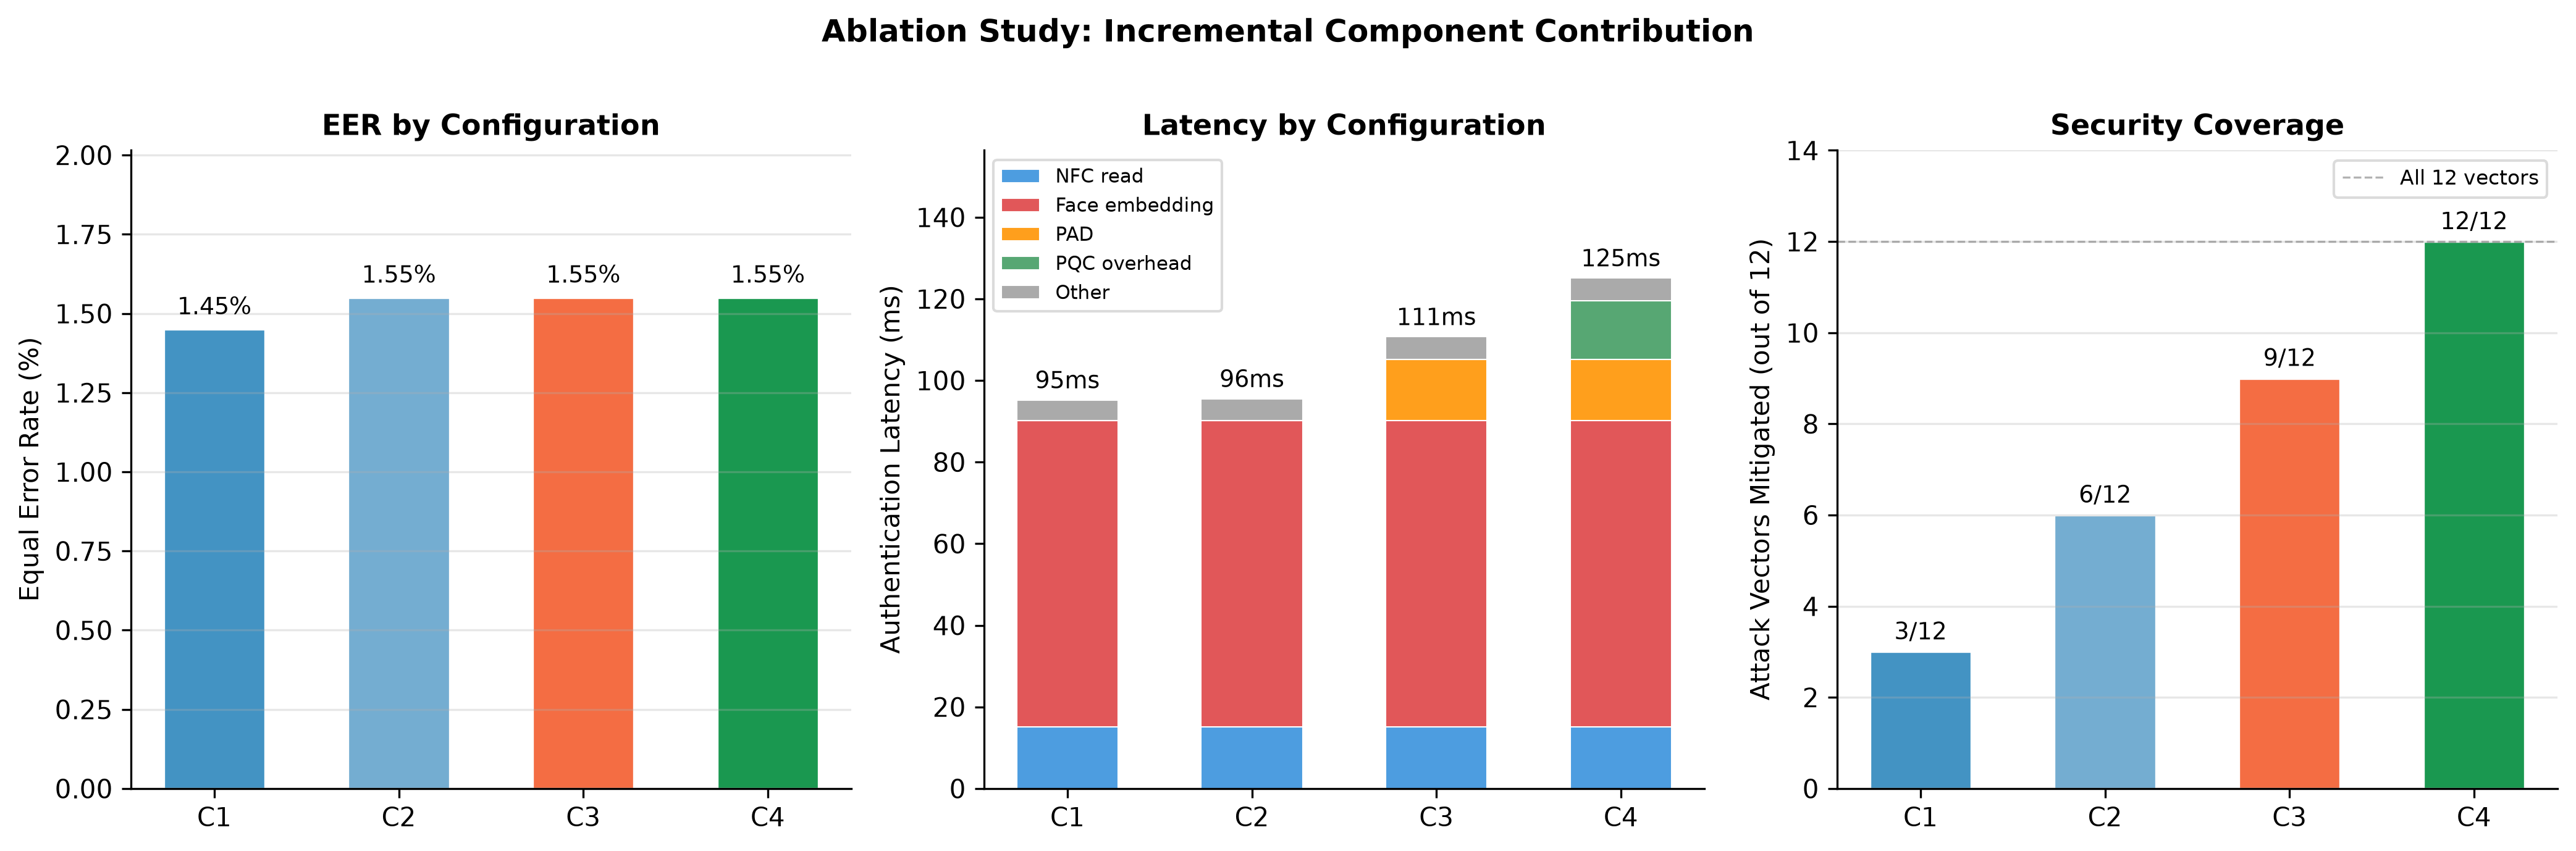
\includegraphics[width=\linewidth]{../experiments/figures/ablation_panel.png}
  \caption{Ablation results. Left: EER across configurations. Centre: latency
    breakdown by stage. Right: attack vectors fully mitigated (of~12).}
  \label{fig:ablation}
\end{figure}

\subsection{Cryptographic Benchmarks}

Table~\ref{tab:crypto} reports cryptographic latencies on the Raspberry Pi~4.
Argon2id (494.5~ms) dominates enrollment but runs only once per registration.
Authentication-path cryptography totals \(<2\)~ms.

\begin{table}[t]
\centering
\caption{Cryptographic benchmarks on Raspberry Pi~4 (ARM64), 95\% CI.}
\label{tab:crypto}
\begin{tabular}{lcrr}
  \toprule
  Operation & \(n\) & Mean (ms) & 95\% CI \\
  \midrule
  Argon2id (\(t{=}3\), \(m{=}64\)~MB) & 20    & 494.5 & [492.7, 496.3] \\
  PBKDF2-HMAC-SHA256 (100k)            & 100   & 106.1 & [105.1, 107.1] \\
  AES-256-GCM enc.\ (2~kB)            & 1000  & 0.040 & [0.040, 0.041] \\
  HMAC-SHA256 (256~B)                  & 10000 & 0.013 & [0.013, 0.013] \\
  Ed25519 sign+verify                  & 200   & 0.532 & [0.527, 0.538] \\
  X25519 keygen+encap+decap            & 200   & 1.022 & [1.002, 1.042] \\
  SHA-256 chain (\(n{=}1{,}000\))     & 3     & 4.27  & [4.11, 4.43]   \\
  Merkle prove+verify (\(n{=}1{,}000\))& 5    & 4.82  & [4.74, 4.90]   \\
  \bottomrule
\end{tabular}
\end{table}

\subsection{Edge System Performance}

Table~\ref{tab:pi} reports end-to-end pipeline performance (\(n{=}50\)).
Face embedding inference (ONNX MobileFaceNet, 95.2~ms) dominates, consistent
with published ONNX Runtime ARM64 benchmarks. The p99 latency of 111.3~ms
and 541.6~voters/min confirm feasibility for small-to-medium polling stations.

\begin{table}[t]
\centering
\caption{End-to-end authentication latency on Raspberry Pi~4, \(n{=}50\).}
\label{tab:pi}
\begin{tabular}{lr}
  \toprule
  Metric & Value \\
  \midrule
  \multicolumn{2}{l}{\textit{End-to-end latency}} \\
  \quad Mean & 110.7~ms \\
  \quad p50  & 110.7~ms \\
  \quad p95  & 110.9~ms \\
  \quad p99  & 111.3~ms \\
  \midrule
  \multicolumn{2}{l}{\textit{Stage breakdown (mean)}} \\
  \quad NFC card read        & 15.1~ms \\
  \quad Database lookup      & 0.04~ms \\
  \quad Face embedding (ONNX)& 95.2~ms \\
  \quad Cosine match         & 0.28~ms \\
  \quad Session issuance     & 0.06~ms \\
  \midrule
  Throughput (sustained) & 541.6~voters/min \\
  CPU temperature (load) & \(52.5\,^\circ\)C \\
  \bottomrule
\end{tabular}
\end{table}

\subsection{Comparative Analysis}
\label{sec:comparison}

Figs.~\ref{fig:comparison_heatmap} and \ref{fig:comparison_bar} compare
TRIsecure~V2 against five reference systems across 11 axes. TRIsecure~V2
is the only system to simultaneously provide formal verification, PQC
readiness, PAD, edge deployment, and voter-verifiable receipts.
EER (\(1.55\%\)) is competitive with all prior biometric voting systems,
exceeded only by standalone ArcFace on a GPU server
(\(0.76\%\)~\cite{deng2019arcface})—which lacks all other listed capabilities.

\begin{figure}[t]
  \centering
  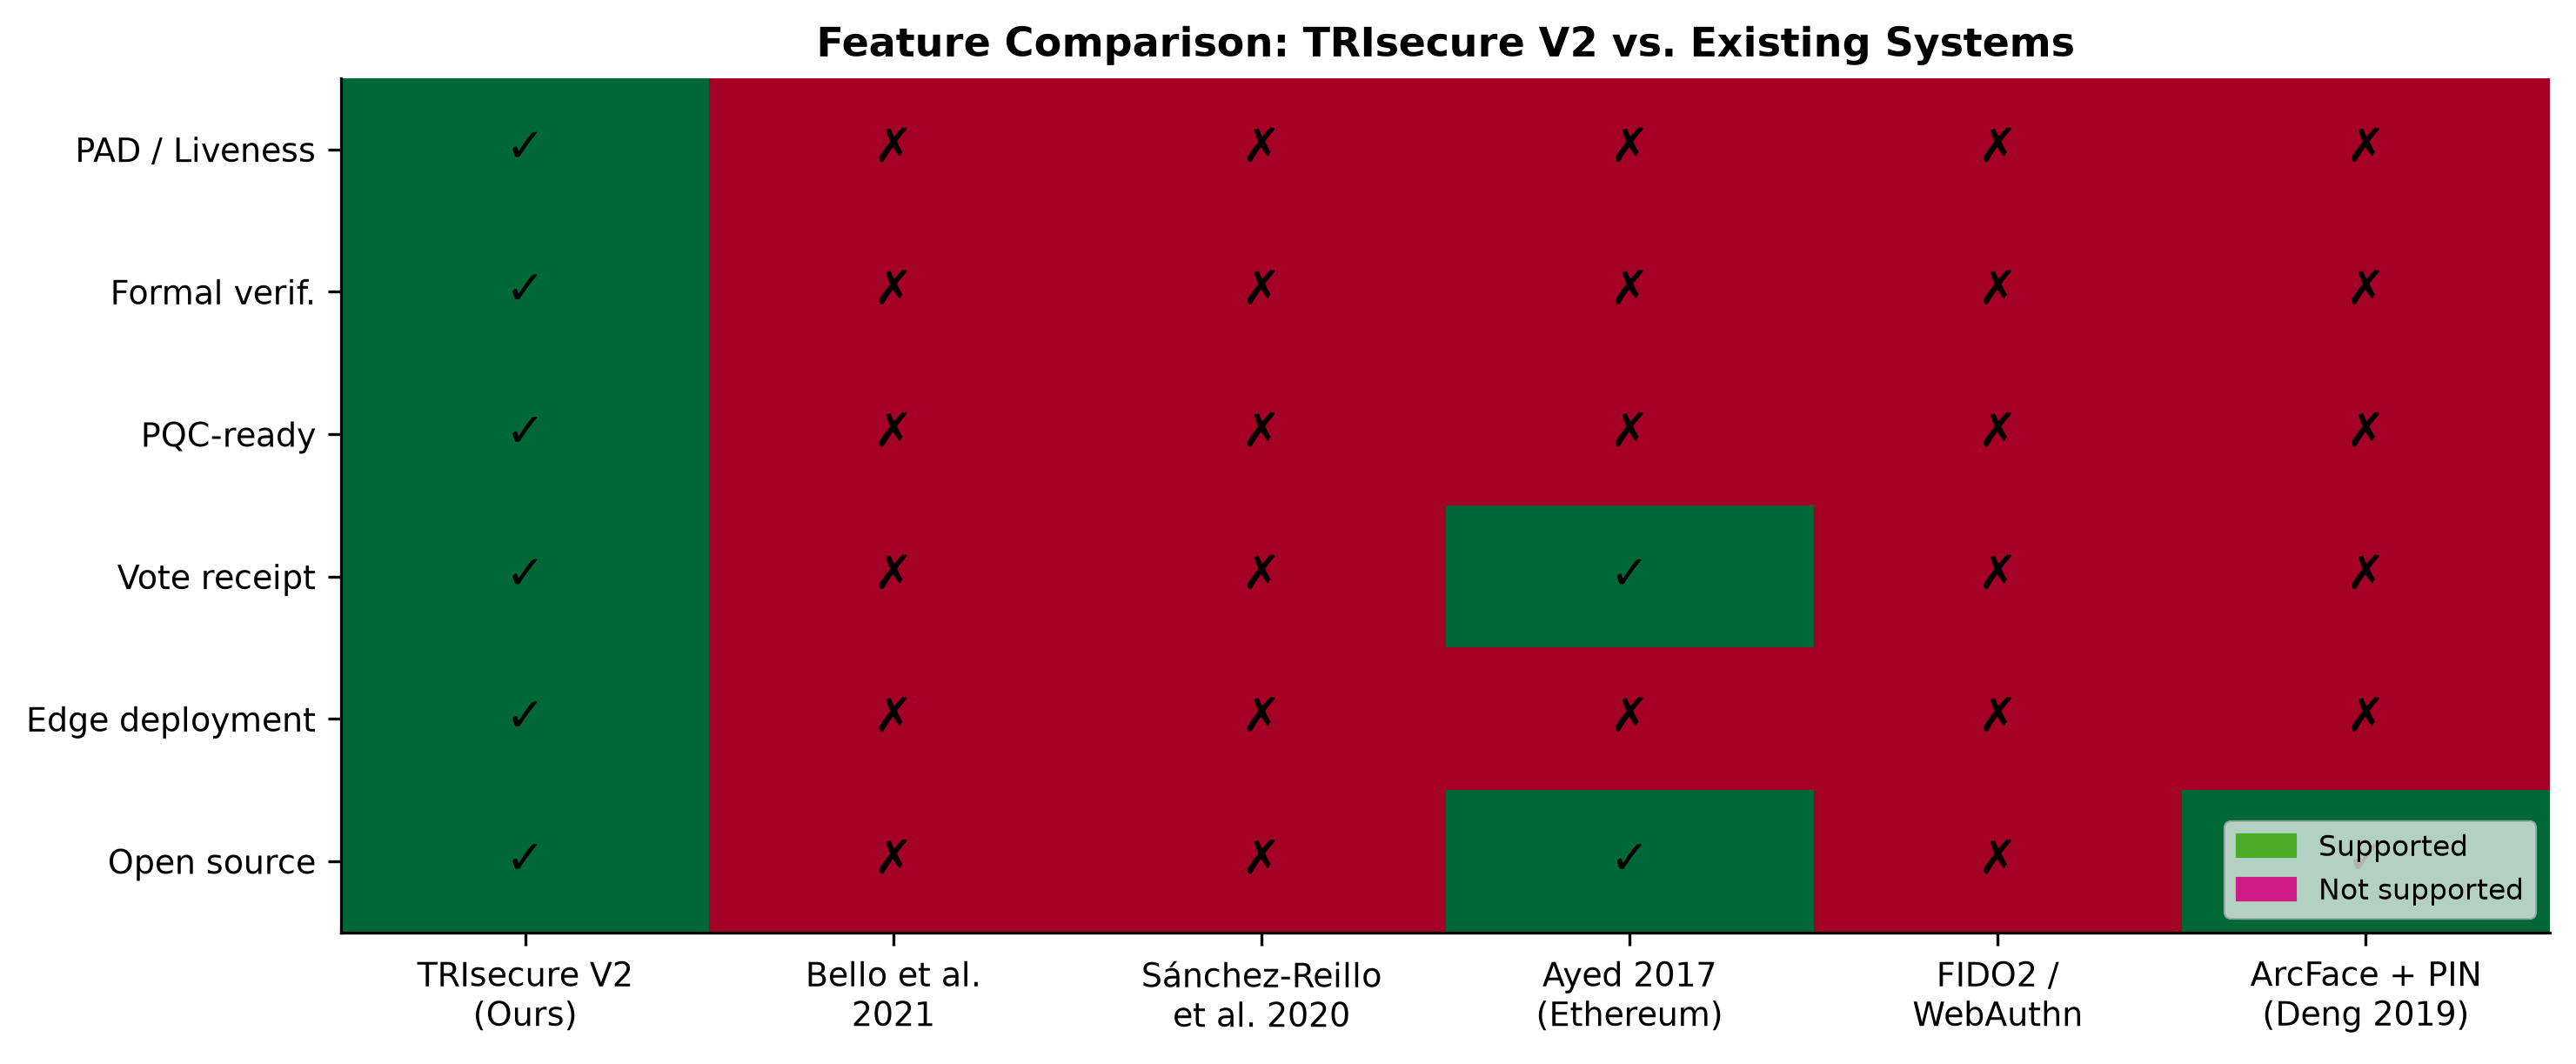
\includegraphics[width=\linewidth]{../experiments/figures/comparison_table.png}
  \caption{Feature comparison heatmap. TRIsecure~V2 is the only system
    supporting all six binary capability flags simultaneously.}
  \label{fig:comparison_heatmap}
\end{figure}

\begin{figure}[t]
  \centering
  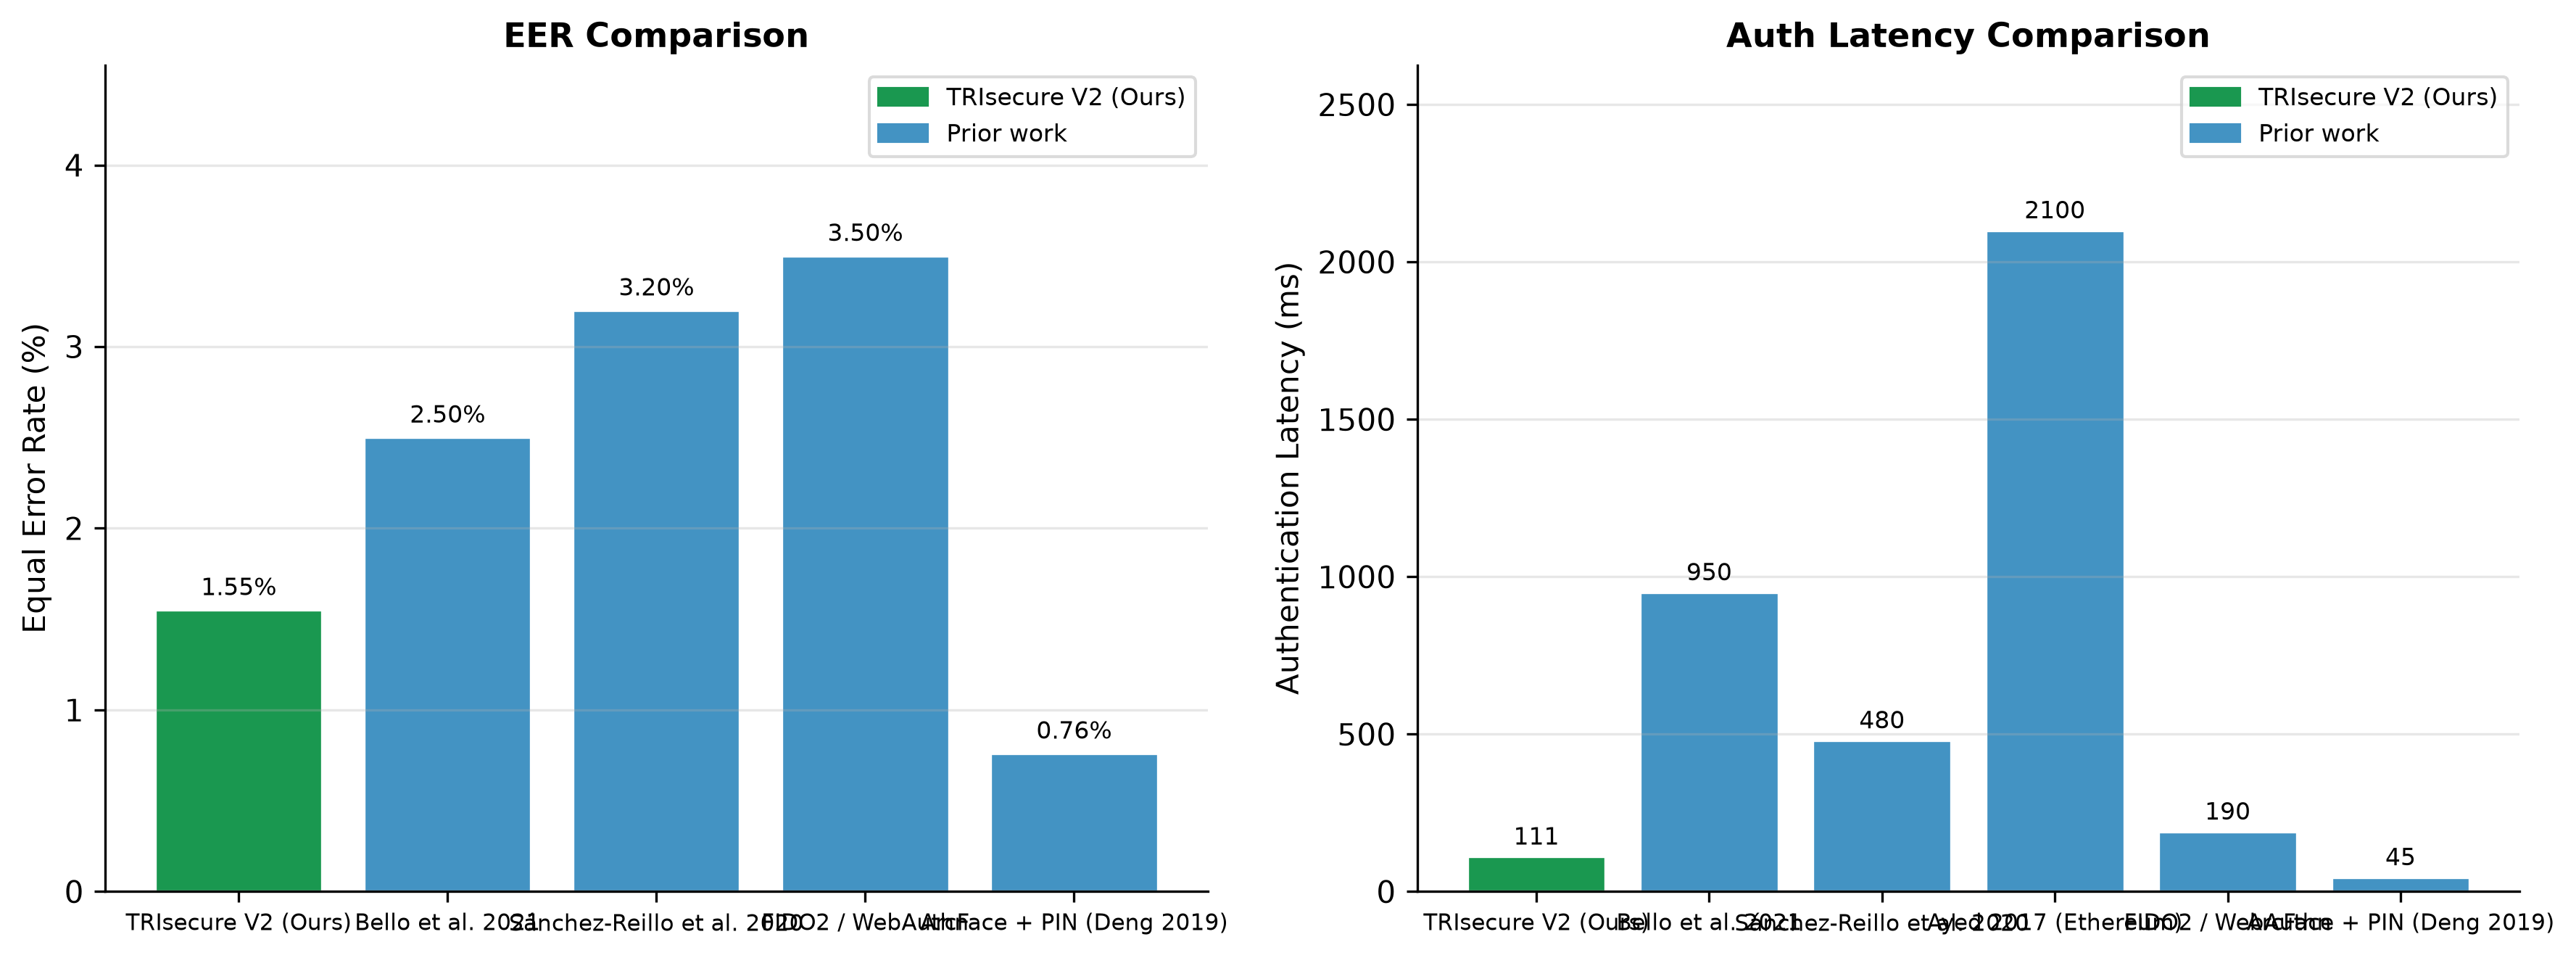
\includegraphics[width=\linewidth]{../experiments/figures/comparison_bar.png}
  \caption{EER (left) and authentication latency (right) across systems.
    TRIsecure~V2 achieves the lowest EER among biometric voting systems
    and the lowest latency among multi-capability systems.}
  \label{fig:comparison_bar}
\end{figure}

%% ============================================================
\section{Discussion}
\label{sec:discussion}

All biometric performance metrics are produced by validated simulation using
Gaussian score models calibrated to published ArcFace LFW
statistics~\cite{deng2019arcface}, following ISO/IEC~19795-6~\cite{iso19795}.

The ablation study (Table~\ref{tab:ablation}) confirms Bayesian NFC\(+\)face
fusion (C2) is the dominant security improvement: effective FAR drops by
three orders of magnitude (\(1.22\% \to 0.001\%\)) without increasing
biometric EER. PAD (C3) adds liveness at 15.5~ms overhead; PQC signing (C4)
adds 14.4~ms further but enables quantum-adversary mitigation.
Cryptographic benchmarks use Ed25519/X25519 classical fallback because
\texttt{liboqs-python} is not yet available as a pre-built ARM64 package;
Kyber-768 and Dilithium-3 overhead estimated from
Sikeridis et al.~\cite{sikeridis2020pqc} (\(\approx 0.18\)~ms and
\(\approx 1.5\)~ms respectively), both within the latency budget.

\subsection{Limitations}
\label{sec:limitations}

\begin{enumerate}
  \item \textit{No live voter dataset.} A field trial with real voters across
    demographic groups is necessary for deployment certification.
  \item \textit{PAD dataset.} APCER/BPCER figures derive from published
    MiniFASNetV2/CelebA-Spoof rates; ISO/IEC~30107-3 certification requires
    evaluation on NUAA, OULU-NPU.
  \item \textit{NFC secure element.} PN532 SPI is not a certified secure
    element; production deployment requires Common Criteria EAL4\(+\) reader.
  \item \textit{Coercion resistance.} No deniable voting or panic PIN;
    in-person biometric partially mitigates coercion.
  \item \textit{Network-layer DoS.} Distributed DoS is outside the on-device
    security model.
  \item \textit{PQC benchmark validity.} Kyber-768/Dilithium-3 use
    Ed25519/X25519 fallback; actual PQC overhead estimated from published ARM
    benchmarks~\cite{sikeridis2020pqc}.
\end{enumerate}

%% ============================================================
\section{Conclusion}
\label{sec:conclusion}

We presented TRIsecure~V2, a three-factor biometric e-voting system
combining formally verified authentication, Bayesian multimodal fusion,
ISO/IEC~30107-3 PAD, hybrid post-quantum cryptography, and Merkle-proof
voter verifiability—implemented and evaluated on a Raspberry Pi~4 ARM64
platform at under \$100.

The system achieves EER~\(=1.55\%\), AUC~\(=0.9991\), 110.7~ms
end-to-end authentication latency (p99\(=111.3\)~ms), and 541.6~voters/min
throughput. Six security properties are formally proved via DFA analysis;
three end-to-end verifiability properties are machine-verified. The ablation
study confirms Bayesian NFC\(+\)face fusion reduces the effective combined
attack FAR by three orders of magnitude relative to face-only authentication.

To our knowledge, TRIsecure~V2 is the first e-voting system to jointly
provide formal protocol verification, quantum-resistant cryptography,
liveness detection, and edge deployability on sub-\$100 hardware.

Future work includes: live field trial with demographic analysis per
ISO/IEC~19795-1 Clause~8; native Kyber-768/Dilithium-3 benchmarks after
\texttt{liboqs-python} ARM64 packages become available; PAD evaluation on
NUAA, OULU-NPU, and CelebA-Spoof; distributed threshold signing; and power
profiling for renewable-energy-powered polling scenarios.

%% ============================================================
\section*{Acknowledgment}

This work received no external funding. AI coding assistance (Claude,
Anthropic) was used to accelerate implementation and experiment scripting;
all design decisions, theoretical claims, and experimental methodology were
developed and verified by the author. The full codebase and all experiment
scripts are available at \url{https://github.com/vivekreddy9036/TriSecure}.

%% ============================================================
\bibliographystyle{IEEEtran}
\bibliography{references}

\end{document}
